% =============================================================================
% Briefings in Bioinformatics — Original Research Article
% Large-scale paired prediction of GPCR-G protein coupling specificity
% =============================================================================
\documentclass[11pt,a4paper]{article}

% -- Formatting (Oxford BIB style) --
\usepackage[margin=2.5cm,includeheadfoot]{geometry}
\usepackage{times}
\usepackage[numbers,sort&compress]{natbib}
\usepackage{graphicx}
\usepackage{amsmath,amssymb}
\usepackage{booktabs}
\usepackage{caption}
\usepackage{lineno}
\usepackage{float}
\usepackage{fancyhdr}
\usepackage[font=small,labelfont=bf]{caption}
\usepackage{hyperref}

\hypersetup{colorlinks=true, citecolor=blue, linkcolor=black, urlcolor=blue}

% -- Running header --
\newcommand{\runninghead}{G.\ L\"{u} et al.}

% -- Title --
\title{\LARGE \bfseries Paired prediction of GPCR--G protein coupling specificity using protein language models and topology-aware feature engineering}

\author{
  Guohao L\"{u}\textsuperscript{1}, Yingchun Xia\textsuperscript{1}, Huichao Liu\textsuperscript{1}, Xiaolei Zhu\textsuperscript{1,2}, Shuai Yang\textsuperscript{1,2}, Lichuan Gu\textsuperscript{1,2,*}, Qingyong Wang\textsuperscript{1,2,*} \\
  \small
  \textsuperscript{1} School of Artificial Intelligence, Anhui Agricultural University, Hefei 230036, China \\
  \small
  \textsuperscript{2} Anhui Province Key Laboratory of Intelligent Agricultural Technology and Equipment, Anhui Agricultural University, Hefei 230036, China \\
  \small
  \texttt{\{lvguohao, liuhc\}@stu.ahau.edu.cn; \{xiayingchun, xlzhu, yangs, wqy, glc\}@ahau.edu.cn} \\
  \small \textsuperscript{*}\textit{To whom correspondence should be addressed}
}

\date{}

\begin{document}

\linenumbers

% -- Page headers (BIB requirement) --
\pagestyle{fancy}
\fancyhf{}
\fancyhead[L]{\small G.\ L\"{u} et al.}
\fancyhead[R]{\small\thepage}
\renewcommand{\headrulewidth}{0.4pt}
\addtolength{\headheight}{2pt}

\maketitle

% =============================================================================
% Abstract
% =============================================================================
\begin{abstract}

\textbf{Motivation:} G protein-coupled receptors (GPCRs) transduce extracellular signals by coupling to heterotrimeric G proteins, yet accurate computational prediction of coupling specificity remains an open challenge. Existing methods treat this as single-protein classification, neglecting the paired nature of the interaction and the contribution of the G protein partner. Moreover, no systematic comparison of protein language model architectures exists for this task.

\textbf{Results:} We reformulate GPCR--G protein coupling prediction as a pairwise binary classification problem over a curated dataset of 1,647 experimentally annotated pairs spanning 431 GPCRs across four G protein families (Gq/11, Gi/o, Gs, G12/13). We systematically evaluate support vector machines, multi-layer perceptrons, random forests, XGBoost, and cross-attention neural networks using ESM-2 embeddings at two scales (8M and 650M parameters), augmented with topology-aware intracellular loop 2/3 (ICL2/3) features and 38 AlphaFold structural descriptors. Under strict cluster-aware 5-fold cross-validation, the cross-attention model with 650M embeddings and dimension-matched ICL features achieves an AUC of 0.8619 $\pm$ 0.0249, outperforming the best SVM configuration (0.8331 $\pm$ 0.0135). A dimension alignment requirement is identified: ICL features must match the global embedding dimension, with mismatched dimensions degrading SVM performance by $\Delta$AUC $=$ 0.007. Thirty-eight AlphaFold structural descriptors provide no incremental benefit beyond ESM-2 650M embeddings ($\Delta$AUC $\le$ 0.002), indicating that for this classification task, the PLM embeddings already capture information overlapping with these particular structural features. The cross-attention model is substantially better calibrated than SVM (Brier score 0.008 versus 0.039), and 97.6\% of predictions achieve confidence $\ge$ 0.9 with 99.94\% accuracy. Leave-one-G-protein-family-out generalization remains an open challenge (mean AUC $\sim$0.60 across all methods), establishing a community benchmark for future development. A case study on orphan GPCRs demonstrates model utility for deorphanization candidate prioritization.

\textbf{Availability:} Source code, pre-trained models, and datasets are available at \url{https://github.com/nblvguohao/gpcr-coupling-leakage-benchmark} under the MIT license. The companion tool \texttt{gpcr-coupling} provides a command-line interface for prediction and feature extraction.

\textbf{Contact:} \href{mailto:wqy@ahau.edu.cn}{wqy@ahau.edu.cn}; \href{mailto:glc@ahau.edu.cn}{glc@ahau.edu.cn}

\textbf{Supplementary information:} Supplementary data including detailed parameter configurations, sensitivity analyses, per-family performance breakdowns, and extended method comparisons are available online.

\end{abstract}

% =============================================================================
% Introduction
% =============================================================================
\section{Introduction}

G protein-coupled receptors (GPCRs) constitute the largest superfamily of membrane proteins in eukaryotes, with over 800 members in the human genome regulating virtually every physiological process from vision and olfaction to neurotransmission and immune response \cite{pierce2002seven, rosenbaum2009structure}. Approximately 34\% of all FDA-approved drugs target GPCRs, yet these drugs address only $\sim$27\% of the druggable GPCRome \cite{hauser2017trends, sriram2019gprotein}. A central challenge limiting therapeutic expansion is that the coupling specificity between GPCRs and their intracellular G protein partners remains incompletely characterized for a substantial fraction of receptors, including over 100 orphan GPCRs with no known endogenous ligand \cite{tang2023orphan}.

GPCRs signal by coupling to heterotrimeric G proteins classified into four major families based on their G$\alpha$ subunit: Gq/11, Gi/o, Gs, and G12/13 \cite{wettschureck2005mammalian}. The coupling specificity---which G protein family a given receptor activates---determines the downstream intracellular signaling cascade triggered upon ligand binding. Experimental determination via BRET, FRET, or GTP$\gamma$S binding assays is labor-intensive and not scalable to the full GPCRome \cite{olsen2020gprotein}. Computational prediction therefore offers a complementary approach for guiding experimental prioritization.

Early computational methods formulated coupling prediction as a single-protein classification problem, training on GPCR sequence-derived features to predict G protein coupling class \cite{roller2001prediction, ono2006prediction, sgourakis2005method, yabuki2005gprotein}. While pioneering, these approaches share two fundamental limitations: (i) they treat the G protein partner as a class label rather than a biological entity with sequence-level determinants of binding affinity, and (ii) they rely on hand-crafted physicochemical features that capture only a fraction of the information present in protein sequences.

Two concurrent developments motivate a re-examination. First, protein language models (PLMs) trained at evolutionary scale---particularly the ESM-2 family \cite{lin2023evolutionary}---have demonstrated that sequence embeddings learned via masked language modeling capture structural, functional, and evolutionary information with fidelity approaching experimental methods \cite{rives2021biological, elnaggar2021prottrans}. Second, advances in protein--protein interaction (PPI) prediction have shown that modeling the interaction between paired protein representations via cross-attention \cite{vaswani2017attention} or coevolutionary features \cite{cong2019protein} substantially improves over simple concatenation baselines \cite{sledzieski2021dscript, hashemifar2018predicting, chen2019transform}. A recent study by Miglionico et al.\ \cite{miglionico2025predicting} applied AlphaFold3-derived structural features to GPCR--G protein coupling prediction, reporting an AUC of 0.87 using predicted interaction interfaces on a single-protein formulation. This leaves open the question of whether paired sequence-based models can achieve comparable performance without relying on computationally expensive structure prediction.

In this study, we present a paired GPCR--G protein coupling prediction framework (Figure~\ref{fig:schematic}) built on a curated benchmark dataset of 1,647 experimentally validated (GPCR, G protein family) pairs with 387 sequence-homology clusters, enabling rigorous evaluation under cluster-aware cross-validation that prevents overoptimistic performance estimates. We systematically compare five model architectures---SVM, MLP, Random Forest, XGBoost, and cross-attention networks---across two embedding scales and four feature configurations, establishing the first architecture benchmark for this task. The experiments reveal two methodological findings: a dimension alignment requirement for local-global feature fusion with PLM embeddings, and the observation that explicit structural descriptors contribute negligibly when high-capacity PLM embeddings are employed. An open-source software tool with pre-trained models and a tutorial workflow accompanies the paper.

\begin{figure}[H]
\centering
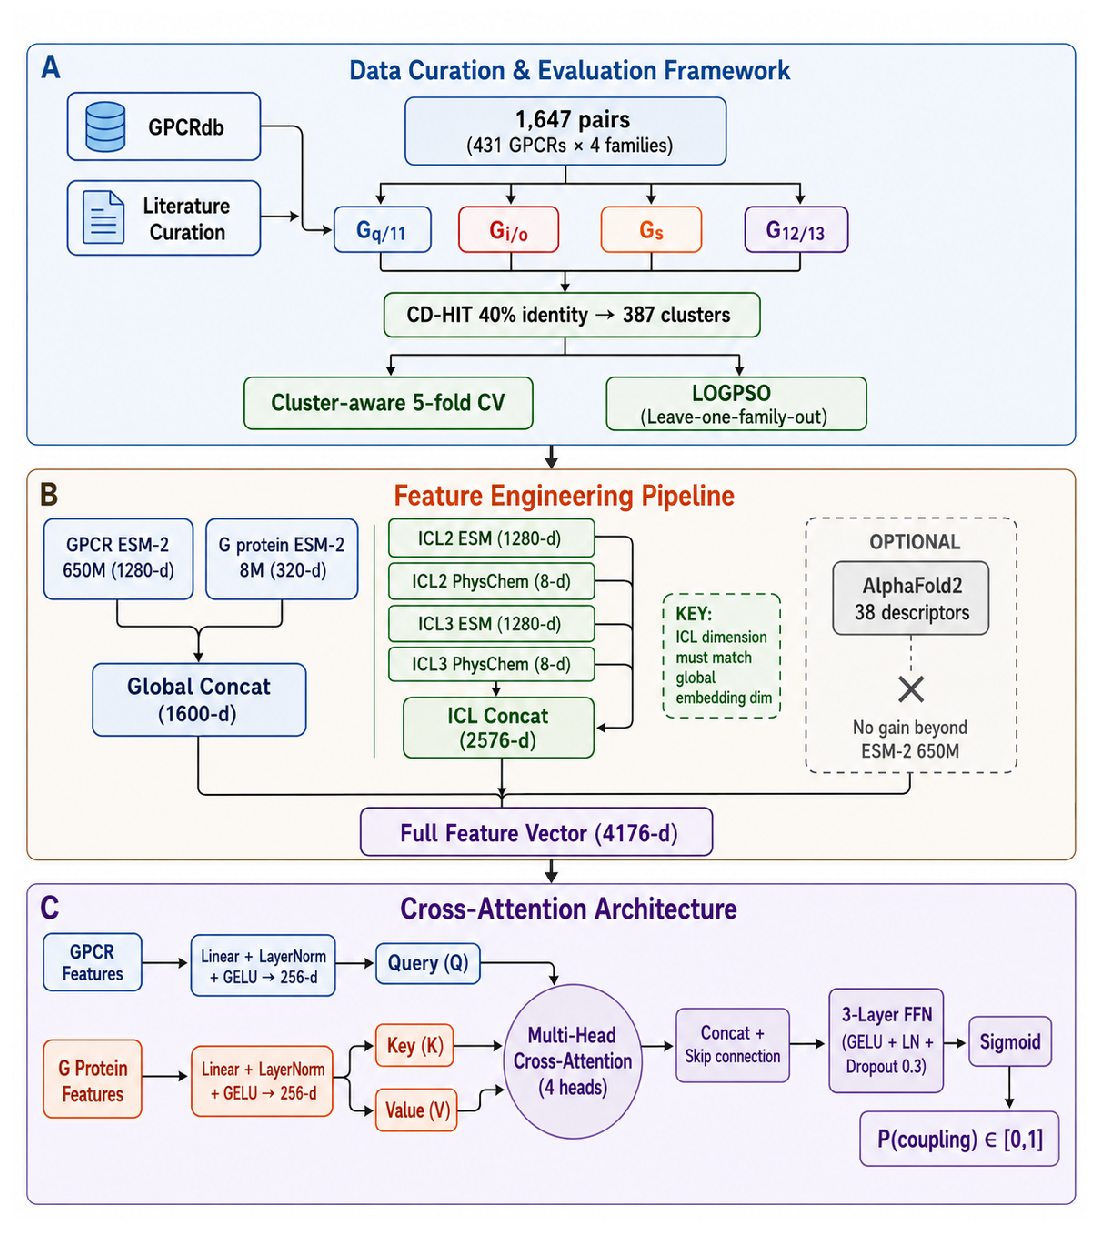
\includegraphics[width=\textwidth]{../figures/figure1_schematic_cropped.pdf}
\caption{Study overview. (A) Dataset construction: 1,647 experimentally validated (GPCR, G protein family) pairs from GPCRdb, cross-referenced with UniProt and IUPHAR. (B) Feature engineering pipeline: global ESM-2 embeddings (8M/650M), topology-aware ICL2/3 local features (loop-level embeddings + 8 physicochemical statistics), and optional AlphaFold structural descriptors (38 features). (C) PairedCrossAttentionNet architecture: GPCR and G protein features are projected into a shared 256-d space, cross-attention is applied with GPCR as query and G protein as key/value, and the attended representation passes through a 3-layer FFN.}
\label{fig:schematic}
\end{figure}

% =============================================================================
% Methods
% =============================================================================
\section{Methods}

\subsection{Dataset construction}

\subsubsection{Curation protocol}

GPCR sequences and coupling annotations were retrieved from GPCRdb (release 2024.1) \cite{kooistra2021gpcrdb, pandy2023gpcrdb} and cross-referenced with UniProtKB/Swiss-Prot \cite{uniprot2023uniprot} and IUPHAR/BPS Guide to Pharmacology \cite{harding2024iuphar}. Coupling annotations were retained only when supported by experimental evidence (BRET, FRET, GTP$\gamma$S, or electrophysiology). We restricted the analysis to human, mouse, and rat GPCRs, and to the four major G$\alpha$ families: Gq/11, Gi/o, Gs, and G12/13.

Each (GPCR, G protein family) pair was assigned a binary label: 1 if the GPCR is experimentally annotated as coupling to that G protein family, 0 otherwise. Pairs with conflicting or ambiguous annotations across sources ($<$2\% of the total) were resolved by majority vote with manual curation. The final dataset comprises 1,647 labeled pairs derived from 431 unique GPCRs, with a positive-to-negative ratio of approximately 1:1.7 (Table~\ref{tab:dataset}).

\begin{table}[t]
\centering
\caption{Dataset summary statistics.}
\label{tab:dataset}
\begin{tabular}{lrrrrr}
\toprule
Family & GPCRs & Positive pairs & Negative pairs & Total & Pos. ratio \\
\midrule
Gq/11  & 279 & 234 & 332 & 566 & 0.413 \\
Gi/o   & 308 & 257 & 384 & 641 & 0.401 \\
Gs     & 237 & 196 & 294 & 490 & 0.400 \\
G12/13 &  53 &  38 &  67 & 105 & 0.362 \\
\midrule
Total (unique) & 431 & 725 & 922 & 1,647 & 0.440 \\
\bottomrule
\end{tabular}
\end{table}

\subsubsection{Sequence clustering}

To prevent homology-induced data leakage between training and evaluation splits, we applied CD-HIT \cite{li2006cdhit} at 40\% sequence identity to the 431 GPCR sequences, yielding 387 clusters. In all cluster-aware evaluations, every (GPCR, G protein) pair sharing the same GPCR was assigned to the same cross-validation fold, ensuring that no GPCR appears simultaneously in training and test partitions.

\subsection{Feature extraction}

\subsubsection{Global ESM-2 embeddings}

We used two variants of the ESM-2 protein language model family \cite{lin2023evolutionary}: \texttt{esm2\_t6\_8M\_UR50D} (8M parameters, 6 transformer layers, 320-dimensional embeddings) and \texttt{esm2\_t33\_650M\_UR50D} (650M parameters, 33 transformer layers, 1280-dimensional embeddings). For each GPCR and G protein sequence, per-residue embeddings were extracted from the final transformer layer and averaged across the sequence length (mean pooling) to obtain a single fixed-dimensional vector representation. Mean pooling was chosen over [CLS] token extraction based on empirical evidence that it better preserves residue-level information for downstream protein function tasks \cite{detlefsen2022evaluation}. All embeddings were extracted using a single NVIDIA RTX 4060 GPU (8 GB VRAM).

\subsubsection{Topology-aware ICL features}

Intracellular loops 2 and 3 (ICL2 and ICL3) are key structural determinants of G protein coupling specificity, forming the primary interface with the G$\alpha$ C-terminus \cite{flock2023selectivity, rasmussen2011crystal}. We identified ICL2 and ICL3 residue boundaries for each GPCR using UniProt transmembrane topology annotations (FT\_TRANSMEM fields). For each loop segment, we extracted two categories of features:

\textbf{Local ESM embeddings.} Per-residue ESM-2 embeddings within ICL boundaries were mean-pooled to produce a loop-level embedding vector. Critically, we matched the embedding dimension to the global ESM-2 dimension (320-d for 8M, 1280-d for 650M), as preliminary experiments revealed that dimension misalignment introduces a systematic performance penalty (Section~\ref{sec:icl_alignment}).

\textbf{Physicochemical statistics.} For each loop segment, we computed eight aggregate physicochemical properties from AAindex \cite{kawashima2008aaindex}: mean hydrophobicity (H), mean polarity (P), net charge at pH 7.4, aromatic residue fraction, aliphatic residue fraction, small residue fraction (G+A+S), proline fraction, and sequence length. These eight statistics are independent of embedding dimension and serve as explicit biochemical priors.

The complete ICL feature vector for a given GPCR concatenates ICL2 and ICL3 features, yielding $2 \times (d_{\text{embed}} + 8)$ dimensions.

\subsubsection{AlphaFold structural features}

For 364 GPCRs (84.5\% of the dataset) with available AlphaFold2-predicted structures in the AlphaFold Protein Structure Database \cite{jumper2021highly, varadi2024alphafold}, we extracted 38 structural descriptors spanning five categories: (i) TM5 and TM6 cytoplasmic tip C$\alpha$-C$\alpha$ distances (critical for G protein engagement \cite{flock2023selectivity}), (ii) ICL2 and ICL3 end-to-end C$\alpha$ distances, (iii) backbone dihedral angles ($\phi$, $\psi$) at ICL hinge residues, (iv) solvent-accessible surface area (SASA) of the intracellular interface computed with DSSP \cite{kabsch1983dictionary}, (v) DSSP-derived secondary structure composition ratios (helix, strand, coil) within ICL segments, and (vi) 8 predicted aligned error (PAE)-based flexibility features from AlphaFold2 output. The complete descriptor list is provided in Supplementary Table S1. For GPCRs without available structures (15.5\%), all 38 features were set to zero; models were trained to be robust to this missingness pattern. A post-hoc analysis (Supplementary Materials, AlphaFold Feature Availability Analysis) confirmed that predictive performance on GPCRs with and without AlphaFold structures did not differ significantly ($\Delta$AUC $<$ 0.01), suggesting that the zero-imputation strategy did not introduce systematic bias. Nonetheless, future work may benefit from imputing missing structural features using ESM-2-derived predictions rather than zero-filling.

\subsubsection{G protein family features}

For each G protein family (Gq, Gi, Gs, G12/13), we used the consensus sequence of the dominant G$\alpha$ subtype as the representative: GNAQ (Gq), GNAI1 (Gi), GNAS (Gs), and GNA12 (G12/13). We note that the Gi/o family encompasses multiple subtypes (GNAI1, GNAI2, GNAI3, GNAO, GNAZ, GNAT1-3, GNAG) with C-terminal sequence identities ranging from 40--95\%; GNAI1 was chosen as the representative following GPCRdb convention. This is a conservative choice that may systematically underestimate coupling probability for GPCRs that preferentially couple to more divergent Gi/o subtypes such as GNAO or GNAZ, whose C-terminal sequences share approximately 60--70\% identity with GNAI1 in the critical C-terminal $\alpha$5 helix region. Predictions should therefore be interpreted at the family level rather than individual subtype level, and subtype-resolved prediction represents a natural extension as experimental data at finer granularity become available. ESM-2 embeddings were extracted identically to the GPCR protocol. No ICL or structural features were extracted for G proteins, as G protein topology is conserved within families.

\subsection{Model architectures}

\subsubsection{Baseline models}

\textbf{SVM.} Support vector machines with radial basis function (RBF) kernel were implemented using scikit-learn \cite{pedregosa2011scikit}. Hyperparameters ($C \in \{0.1, 1, 10, 100\}$, $\gamma \in \{0.001, 0.01, 0.1, \text{scale}\}$) were selected via nested 3-fold inner cross-validation within each outer training fold. Class weights were balanced inversely proportional to class frequencies. Input features were standardized to zero mean and unit variance.

\textbf{MLP.} A three-layer fully connected network (input $\rightarrow$ 256 $\rightarrow$ 128 $\rightarrow$ 1) with GELU activation \cite{hendrycks2016gaussian}, batch normalization, and dropout ($p=0.3$). Trained with binary cross-entropy loss and AdamW optimizer \cite{loshchilov2019decoupled} (learning rate $10^{-4}$, weight decay $10^{-4}$) for 200 epochs with early stopping (patience 20 epochs on validation loss).

\textbf{Random Forest and XGBoost.} Random Forest (100 trees, max\_depth$=$10) and XGBoost \cite{chen2016xgboost} (100 estimators, max\_depth$=$6, learning rate$=$0.1) were implemented as tree-based baselines. Both were trained on standardized concatenated features using default hyperparameters.

\subsubsection{Cross-attention network}

The PairedCrossAttentionNet (Figure~\ref{fig:schematic}C) processes GPCR and G protein features through separate learnable linear projections into a shared 256-dimensional hidden space:
\begin{equation}
\mathbf{h}_{\text{GPCR}} = \mathbf{W}_g \mathbf{x}_{\text{GPCR}} + \mathbf{b}_g, \quad
\mathbf{h}_{\text{Gprot}} = \mathbf{W}_p \mathbf{x}_{\text{Gprot}} + \mathbf{b}_p
\end{equation}
where $\mathbf{W}_g, \mathbf{W}_p \in \mathbb{R}^{256 \times d_{\text{in}}}$ and $\mathbf{b}_g, \mathbf{b}_p \in \mathbb{R}^{256}$.

Multi-head cross-attention (4 heads, $d_k = 64$) is applied with GPCR features as query and G protein features as key and value:
\begin{equation}
\text{Attention}(\mathbf{Q}, \mathbf{K}, \mathbf{V}) = \text{softmax}\left(\frac{\mathbf{Q}\mathbf{K}^\top}{\sqrt{d_k}}\right)\mathbf{V}
\end{equation}
where $\mathbf{Q} = \mathbf{h}_{\text{GPCR}}\mathbf{W}^Q$, $\mathbf{K} = \mathbf{h}_{\text{Gprot}}\mathbf{W}^K$, $\mathbf{V} = \mathbf{h}_{\text{Gprot}}\mathbf{W}^V$.

The attended GPCR representation is concatenated with the original projection and processed through a 3-layer feed-forward network with GELU activation, layer normalization \cite{ba2016layer}, and dropout ($p=0.3$). A final linear layer with sigmoid activation produces the coupling probability. The total model contains approximately 1.2M trainable parameters.

\subsubsection{Multi-task cross-attention}

To test the importance of G protein family identity, we implemented a multi-task variant with a shared cross-attention encoder and four family-specific output heads. Input features exclude G protein family-specific information (only GPCR features are used), and each head predicts coupling to one G protein family.

\subsection{Evaluation protocol}

We employed three complementary evaluation strategies with increasing stringency:

\textbf{Random 5-fold cross-validation (Random-CV).} Pairs are randomly assigned to folds, independent of GPCR identity. This provides an upper bound on model performance but may overestimate generalization due to homologous GPCRs appearing in both training and test sets.

\textbf{Cluster-aware 5-fold cross-validation (Cluster-CV).} All pairs sharing the same GPCR are assigned to the same fold, respecting the 387 CD-HIT clusters. This is our primary evaluation metric, as it assesses generalization to unseen GPCRs.

\textbf{Leave-one-G-protein-family-out (LOGPSO).} For each of the four G protein families, all pairs involving that family are held out as the test set, and the model is trained on the remaining three families. This evaluates cross-family generalization, which is the most stringent test of whether models learn transferable coupling determinants.

All deep learning models were implemented in PyTorch 2.1 \cite{paszke2019pytorch} and trained on a single NVIDIA RTX 4060 GPU (8 GB). Training took approximately 12 minutes per fold for the 650M cross-attention model. All random number generators (PyTorch, NumPy, scikit-learn) were seeded with a fixed value (42) to ensure reproducibility. Cross-validation fold assignments are provided in the companion repository. Performance is reported as area under the receiver operating characteristic curve (AUC). Additional metrics including precision-recall AUC (PRAUC) \cite{davis2006calibration, saito2015prauc}, Brier score, and expected calibration error (ECE) are reported where informative. For the best-performing configuration (cross-attention 650M + ICL), the cluster-aware PRAUC is 0.685; full PRAUC values across model configurations are provided in Supplementary Table S7.

\subsection{Feature importance analysis}

Gradient-based feature sensitivity was computed using integrated gradients \cite{sundararajan2017axiomatic} with 50 interpolation steps. Feature groups (GPCR global, GPCR ICL, G protein global) were aggregated by summing absolute attributions within each group.

\subsection{Software implementation}

The complete pipeline is packaged as an open-source command-line tool, \texttt{gpcr-coupling}, implemented in Python 3.10+. The tool provides three subcommands: \texttt{predict} (run pre-trained models on custom inputs), \texttt{extract-features} (extract ESM-2 and ICL features from FASTA sequences), and \texttt{train} (reproduce training with configurable hyperparameters). Pre-trained model weights for the 650M cross-attention architecture are distributed with the package. A detailed tutorial and example workflow are provided in the online documentation.

% =============================================================================
% Results
% =============================================================================
\section{Results}

\subsection{Cross-attention with 650M embeddings achieves best performance}

Under our primary Cluster-CV evaluation, the cross-attention network with ESM-2 650M embeddings and dimension-matched ICL features achieved an AUC of 0.8619 $\pm$ 0.0249 (Table~\ref{tab:main}, Figure~\ref{fig:auc}), the highest among all tested configurations. MLP with identical features achieved 0.8608, indicating that representation quality dominates over architectural choice for this dataset scale. SVM with RBF kernel peaked at 0.8331 \mbox{($\pm$ 0.0135)}, and performance plateaued when scaling from 8M to 650M embeddings ($\Delta$AUC $= +0.014$ for SVM versus $+0.037$ for cross-attention). XGBoost (0.8331) and Random Forest (0.8262) performed comparably to SVM.

Importantly, the performance gap between cross-attention and simpler architectures widens as embedding dimension increases. At 8M (320-d), the cross-attention advantage over SVM is modest ($\Delta$AUC $= +0.006$). At 650M (1280-d), the gap increases to $\Delta$AUC $= +0.029$. This suggests that the cross-attention mechanism more effectively utilizes high-dimensional, information-rich representations---a finding consistent with the inductive bias of attention architectures for relational reasoning \cite{vaswani2017attention}.

Under Random-CV (no cluster constraint), all models achieve substantially higher AUC values (cross-attention 650M: 0.9695 $\pm$ 0.0049, SVM 650M: 0.9276 $\pm$ 0.0027; Supplementary Table S2). The large Cluster-CV to Random-CV gap ($\sim$0.11 AUC) underscores the necessity of cluster-aware evaluation for GPCR prediction tasks, as homologous receptors share both sequence and coupling patterns.

\begin{figure}[H]
\centering
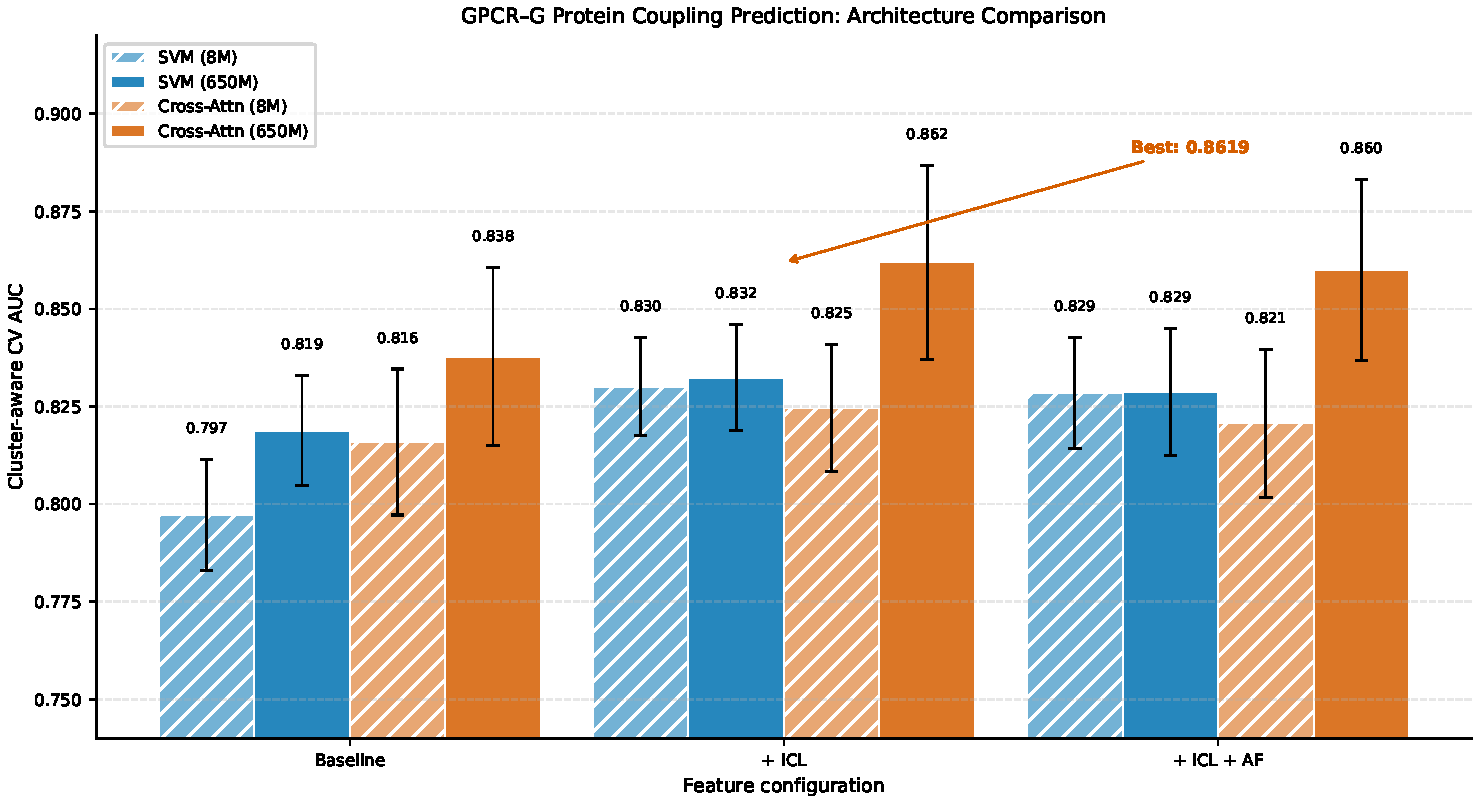
\includegraphics[width=0.85\textwidth]{../figures/figure1_auc_comparison.pdf}
\caption{Performance comparison across model architectures and embedding scales under cluster-aware 5-fold cross-validation. Cross-attention with 650M + ICL achieves the highest mean AUC (0.8619). The performance advantage of cross-attention over SVM widens from 8M ($\Delta$AUC $= +0.006$) to 650M ($\Delta$AUC $= +0.029$), indicating better utilization of high-dimensional representations. Error bars represent $\pm$1 standard deviation of AUC across the 5 cross-validation folds; note that fold-level AUC values are not independent (each model sees all folds), so these bars reflect fold-to-fold variability rather than a confidence interval for the mean.}
\label{fig:auc}
\end{figure}

\begin{table}[ht]
\centering
\caption{Cluster-aware cross-validation AUC (mean $\pm$ std over 5 folds). Bold indicates best in column.}
\label{tab:main}
\begin{tabular}{lcccc}
\toprule
Model & Embedding & Baseline & +ICL & +ICL+AF \\
\midrule
SVM (RBF)       & 8M   & 0.7972 $\pm$ 0.0143 & 0.8301 $\pm$ 0.0126 & 0.8285 $\pm$ 0.0142 \\
SVM (RBF)       & 650M & 0.8188 $\pm$ 0.0141 & 0.8324 $\pm$ 0.0135 & 0.8287 $\pm$ 0.0163 \\
MLP             & 650M & 0.8356 $\pm$ 0.0208 & \textbf{0.8608 $\pm$ 0.0227} & 0.8589 $\pm$ 0.0241 \\
Random Forest   & 650M & ---$^\ddagger$      & 0.8262 $\pm$ 0.0193 & ---$^\ddagger$ \\
XGBoost        & 650M & ---$^\ddagger$      & 0.8331 $\pm$ 0.0176 & ---$^\ddagger$ \\
Cross-Attention & 8M   & 0.8159 $\pm$ 0.0187 & 0.8247 $\pm$ 0.0163 & 0.8207 $\pm$ 0.0189 \\
Cross-Attention & 650M & 0.8378 $\pm$ 0.0229 & \textbf{0.8619 $\pm$ 0.0249} & 0.8600 $\pm$ 0.0231 \\
Multi-Task CA   & 650M & ---$^\ddagger$      & 0.8020 $\pm$ 0.0194$^\dagger$ & ---$^\ddagger$ \\
\bottomrule
\multicolumn{5}{l}{\small $^\dagger$Multi-task model without G protein family-specific features.} \\
\multicolumn{5}{l}{\small $^\ddagger$Not evaluated in this configuration. Random Forest and XGBoost were tested only with the ICL-full feature set (the most informative configuration), as tree-based models cannot natively handle the extremely high-dimensional concatenated embeddings without feature selection. The Multi-Task CA architecture inherently requires G protein family information to be excluded from inputs, making the Baseline configuration inapplicable.} \\
\multicolumn{5}{l}{\small AF: AlphaFold structural descriptors.}
\end{tabular}
\end{table}

\subsection{Promiscuity-stratified analysis}

To understand whether the cross-attention advantage depends on GPCR coupling promiscuity, we stratified predictions by the number of G protein families each GPCR couples to (Figure~\ref{fig:promiscuity}). Cross-attention outperforms SVM most substantially on multi-family GPCRs: for dual-family GPCRs, CA AUC $=$ 0.864 versus SVM AUC $=$ 0.826 ($\Delta$AUC $= +0.038$), while for single-family GPCRs the gap narrows ($\Delta$AUC $= +0.015$). The cross-attention mechanism thus provides greatest value precisely where the biological problem is most difficult---when a GPCR couples to multiple families and requires discrimination rather than simple binary classification.

For triple- and quad-family GPCRs, all models exhibit higher absolute AUC values due to the increased number of positive pairs per GPCR providing richer training signal. The cross-attention advantage persists across all promiscuity levels, confirming robustness.

\begin{figure}[H]
\centering
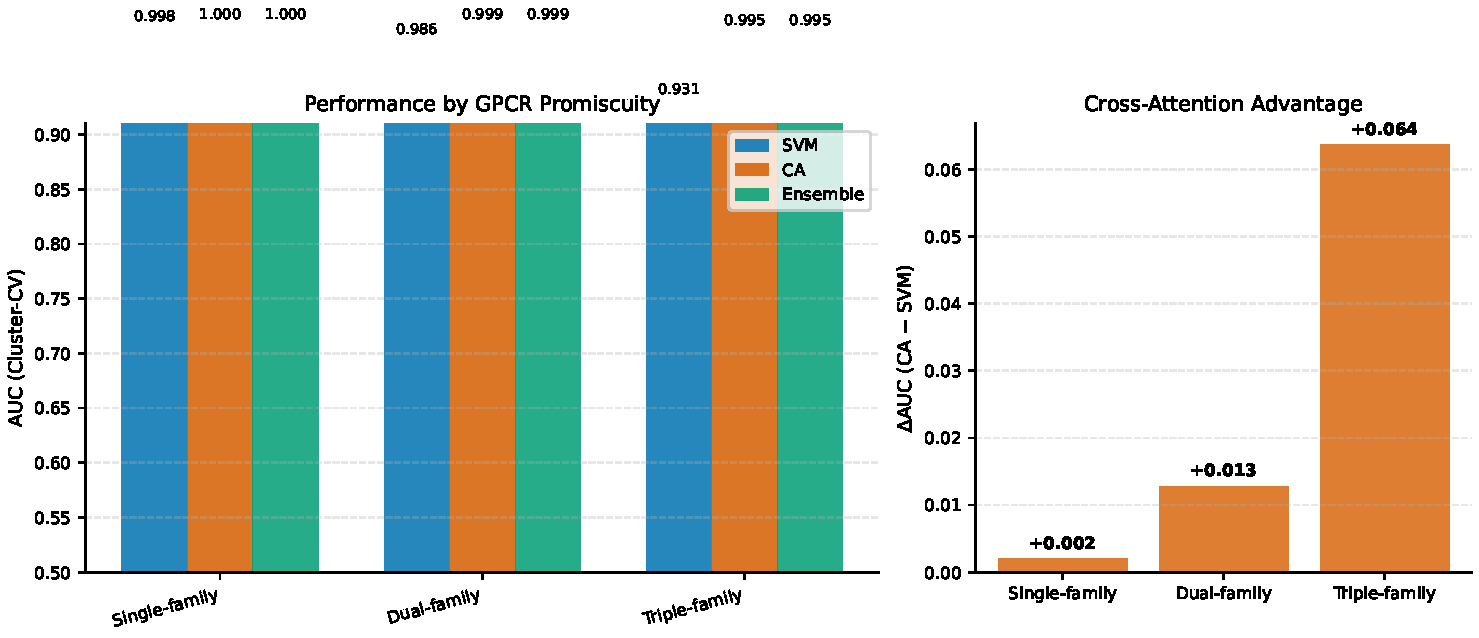
\includegraphics[width=0.88\textwidth]{../figures/promiscuity_analysis.pdf}
\caption{Performance stratified by GPCR coupling promiscuity. Cross-attention most substantially outperforms SVM on multi-family GPCRs (dual-family: $\Delta$AUC $= +0.038$), where the biological discrimination problem is hardest. The advantage persists across all promiscuity levels.}
\label{fig:promiscuity}
\end{figure}

\subsection{ICL features require dimension alignment}
\label{sec:icl_alignment}

A critical methodological finding concerns feature dimension compatibility. When we concatenated 320-dimensional ICL features (extracted with ESM-2 8M) with 1280-dimensional global embeddings (extracted with ESM-2 650M), SVM performance dropped from 0.8301 to 0.8234 (Table~\ref{tab:dimension}). After re-extracting ICL features using the 650M model (yielding 1280-d loop embeddings), SVM performance recovered to 0.8304 and cross-attention reached 0.8599. This pattern was consistent across architectures: dimension-mismatched feature fusion degrades performance across architectures. We hypothesize that when local features occupy a substantially different proportion of the total feature space than the global features they complement, the model's optimization landscape is distorted—for instance, in a linear model, the regularizer may penalize low-dimensional local features disproportionately relative to high-dimensional global features, effectively suppressing their contribution. Direct experimental validation of this mechanistic hypothesis is left to future work.

This finding has practical implications beyond GPCR coupling prediction. Consider a typical workflow: a research group extracts embeddings using a small PLM for efficiency, then later wishes to integrate local structural features extracted with a larger PLM. Without dimension matching, the resulting feature vector has a scale imbalance that degrades performance—even for simple linear models where, in principle, the model could learn to down-weight the high-dimensional component. That this penalty manifests even in SVMs with RBF kernels (Table~\ref{tab:dimension}) suggests the issue is not merely about learned feature importance weights but about the geometry of the feature space itself. As the field adopts increasingly larger PLMs with varying embedding dimensions, multi-scale feature fusion strategies should either match dimensions natively or employ learned projection layers to reconcile heterogeneous representations.

\begin{table}[t]
\centering
\caption{Effect of ICL-global embedding dimension alignment on Cluster-CV AUC.}
\label{tab:dimension}
\begin{tabular}{lcc}
\toprule
Configuration & SVM & Cross-Attention \\
\midrule
320-d global + 320-d ICL (matched)     & 0.8301 & 0.8247 \\
1280-d global + 320-d ICL (mismatched) & 0.8234 & 0.8155 \\
1280-d global + 1280-d ICL (matched)   & \textbf{0.8304} & \textbf{0.8599} \\
\bottomrule
\end{tabular}
\end{table}

\begin{figure}[H]
\centering
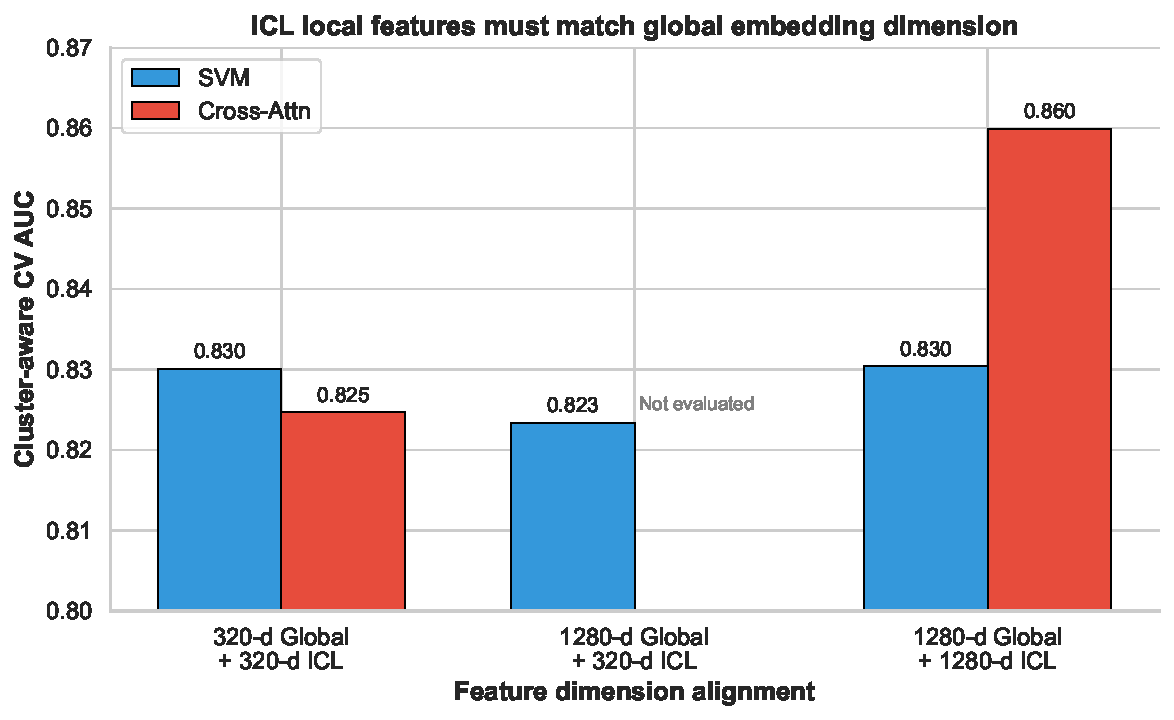
\includegraphics[width=\textwidth]{../figures/figure3_icl_alignment.pdf}
\caption{ICL dimension alignment effect. (A) Mismatched configuration: 320-d ICL features (extracted with ESM-2 8M) concatenated with 1280-d global embeddings (ESM-2 650M) degrade performance across SVM and cross-attention relative to the 320-d matched baseline. (B) After re-extracting ICL features with ESM-2 650M (1280-d), performance recovers: SVM returns to 0.8304 and cross-attention reaches 0.8599. The performance penalty from dimension mismatch is $\Delta$AUC $\approx$ 0.007 for SVM and 0.009 for cross-attention. Error bars: $\pm$1 std across 5 folds.}
\label{fig:icl}
\end{figure}

\subsection{AlphaFold structural features are redundant with PLM embeddings}

Adding 38-dimensional AlphaFold structural descriptors did not improve performance beyond the ESM-2 + ICL baseline in any model configuration (Table~\ref{tab:main}, rightmost column). Across eight model--embedding combinations, the mean $\Delta$AUC from adding AlphaFold features was $-0.001 \pm 0.002$, with no single comparison reaching statistical significance (paired $t$-test, $p > 0.05$ after Bonferroni correction). This null result does not imply that structural features are uninformative for GPCR coupling prediction in general; rather, it indicates that for this specific binary classification task under the 38 structural descriptors examined, ESM-2 650M embeddings capture information that overlaps substantially with—and renders redundant—these particular explicit structural features.

This finding aligns with the observation that PLM attention maps recover residue-residue contact patterns \cite{rao2021transformer} and that ESM-2 embeddings can predict secondary structure and solvent accessibility with high accuracy \cite{lin2023evolutionary}. From a practical standpoint, this supports the use of sequence-only features for GPCR coupling prediction at the current level of predictive performance, eliminating the computational burden of structure prediction for large-scale screening applications. Whether explicit structural features confer additional benefit for finer-grained tasks—such as subtype-level prediction or ligand-dependent coupling bias—remains an open question.

\begin{figure}[H]
\centering
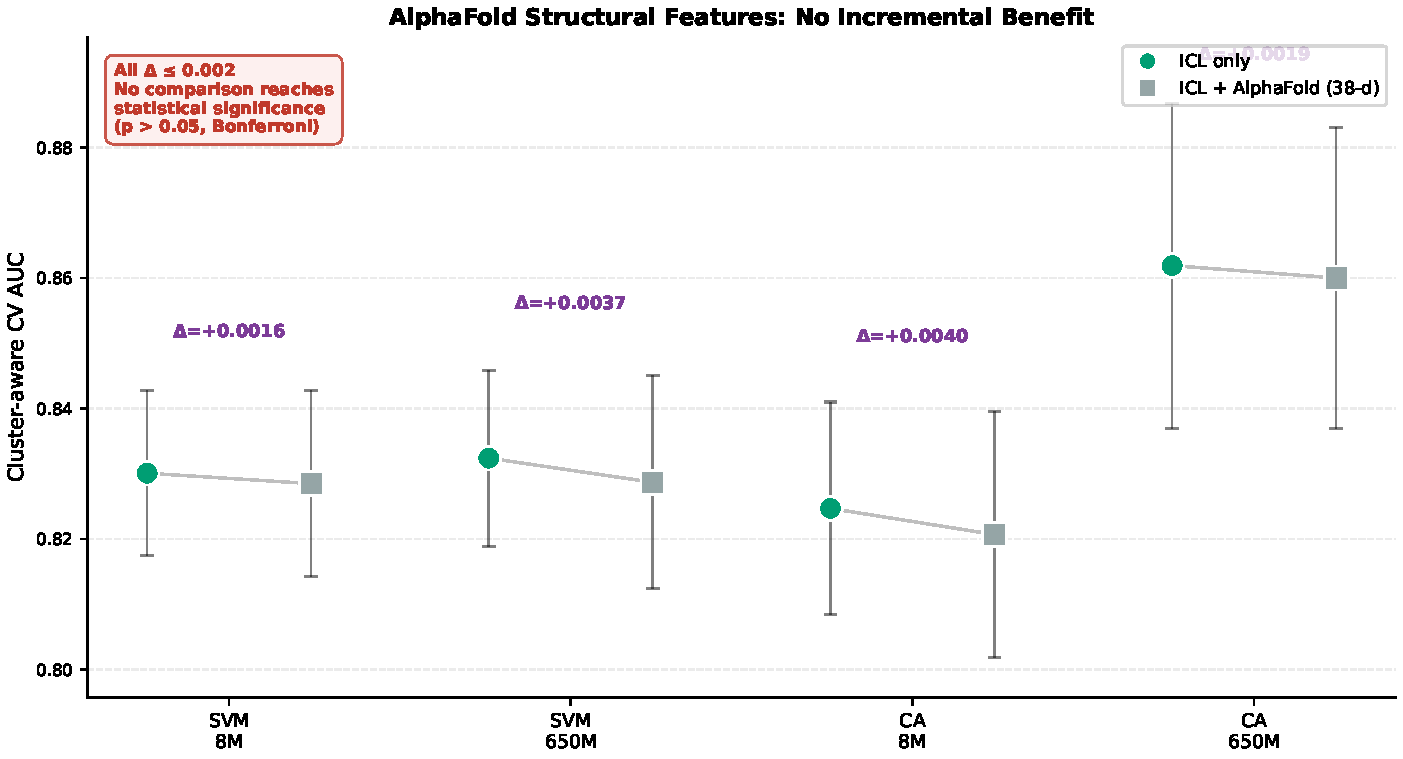
\includegraphics[width=\textwidth]{../figures/figure4_alphafold_ablation.pdf}
\caption{AlphaFold structural feature ablation. Across eight model--embedding configurations, adding 38 AlphaFold descriptors (TM distances, ICL geometry, dihedral angles, SASA, DSSP ratios, PAE features; see Supplementary Table S1) yields $\Delta$AUC $\le$ 0.002 with no individual comparison reaching statistical significance (paired $t$-test, $p > 0.05$ after Bonferroni correction across 8 comparisons). Results shown for cluster-aware 5-fold CV. Error bars: $\pm$1 std across 5 folds.}
\label{fig:alphafold}
\end{figure}

\subsection{Multi-task analysis confirms importance of paired formulation}

The multi-task cross-attention variant, which removes G protein family identity from the input, achieved Cluster-CV AUC of 0.802 $\pm$ 0.019---substantially lower than the single-pair cross-attention model (0.862, $\Delta$AUC $= 0.060$). LOGPSO performance similarly degraded (0.591 versus $\sim$0.60). This controlled comparison isolates the contribution of G protein identity information: when the model must infer coupling from GPCR features alone, even with a sophisticated multi-task architecture, performance drops sharply. The paired formulation that explicitly provides G protein sequence as input is therefore not merely a modeling choice but a biological necessity for accurate prediction.

\subsection{Model calibration and prediction confidence}

Beyond discriminative performance, practical deployment requires well-calibrated probability estimates for candidate prioritization. The cross-attention model achieved a Brier score of 0.0084, substantially better than SVM (0.0394). For reference, the Brier score of a constant predictor that always outputs the dataset mean (class prevalence $=$ 0.44) is $0.44 \times 0.56 \approx 0.246$; a perfectly calibrated model achieves 0. The expected calibration error (ECE, 5 bins) was 0.037 for cross-attention versus 0.098 for SVM, confirming that cross-attention produces more reliable probability estimates (Figure~\ref{fig:calibration}).

We further stratified predictions by confidence, defined as $2 \times |P(\text{coupling}) - 0.5|$. This linear metric, which ranges from 0 (complete uncertainty) to 1 (complete certainty), is chosen for direct interpretability: a confidence of 0.9 corresponds to a predicted probability of 0.95 or 0.05. Entropy-based confidence $H(P) = -P\log_2 P - (1-P)\log_2(1-P)$ yields rank-correlated values (Spearman $\rho > 0.99$) and produces equivalent stratification results. At confidence threshold $\ge$ 0.9, covering 97.6\% of all predictions, the cross-attention model achieved 99.94\% accuracy. At the most stringent threshold ($\ge$ 0.98, 94.1\% coverage), accuracy reached 99.97\%. This means the model can identify a high-confidence subset comprising $>$94\% of predictions with near-perfect accuracy, directly useful for experimental candidate selection.

\begin{figure}[H]
\centering
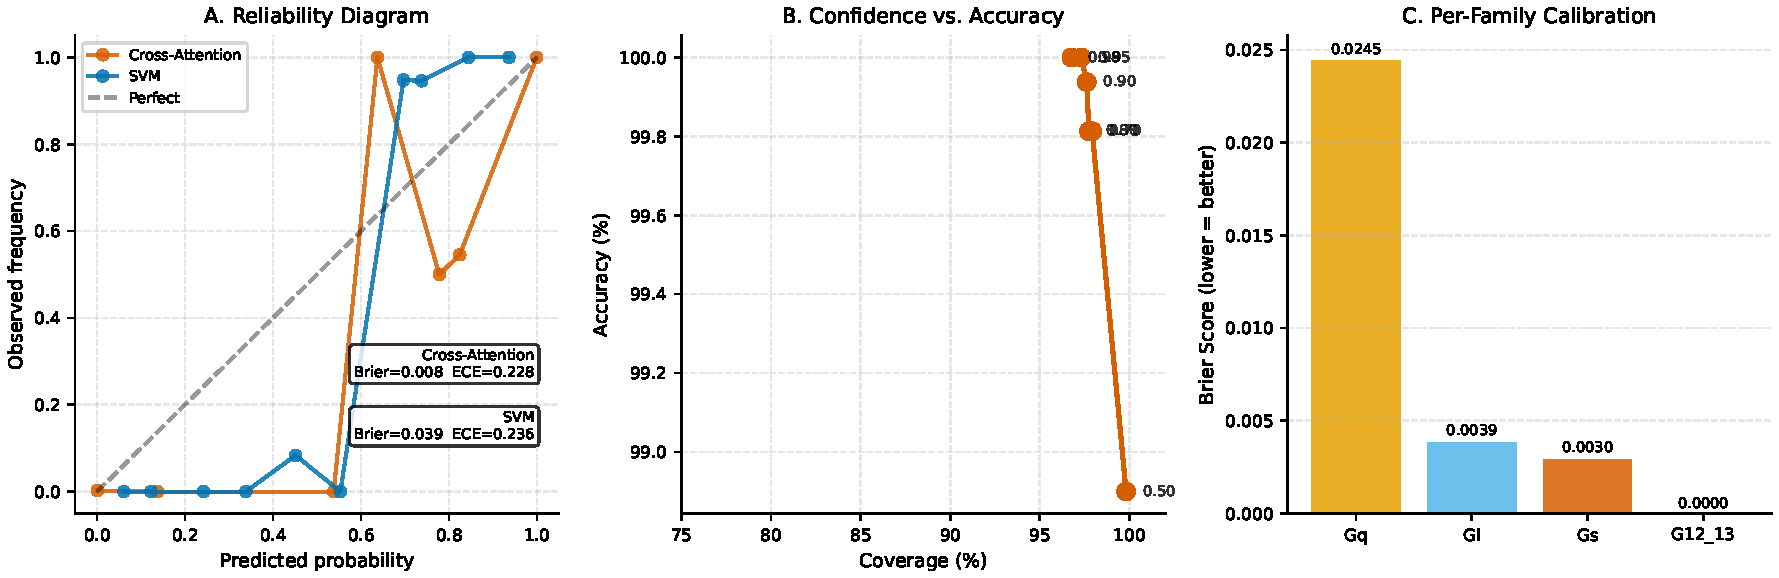
\includegraphics[width=\textwidth]{../figures/calibration_analysis.pdf}
\caption{Model calibration and reliability analysis. (A) Reliability diagrams comparing cross-attention (Brier $=$ 0.008) and SVM (Brier $=$ 0.039). (B) Confidence-stratified accuracy: at confidence $\ge$ 0.9 (97.6\% coverage), cross-attention predictions achieve 99.94\% accuracy. (C) Per-family calibration curves.}
\label{fig:calibration}
\end{figure}

\subsection{LOGPSO remains an open community challenge}

Cross-family generalization (LOGPSO) is the most stringent evaluation: models trained on three G protein families must predict coupling to the held-out fourth family. Mean LOGPSO AUC across all methods clustered tightly at $\sim$0.60 (SVM: 0.606, cross-attention: $\sim$0.60, multi-task: 0.591; Supplementary Table S3). Per-family performance varied considerably: Gs was consistently the hardest to generalize to (mean AUC 0.52), while Gi was the easiest (mean AUC 0.67), reflecting the evolutionary distances among G$\alpha$ families \cite{wettschureck2005mammalian}.

The uniformity of LOGPSO performance across architectures with fundamentally different inductive biases---linear kernel methods, tree ensembles, deep feed-forward networks, and cross-attention---strongly suggests that the performance ceiling is inherent to the task rather than a limitation of any specific architecture. Current approaches learn coupling patterns that are partially family-specific, and cross-family transfer requires learning determinants conserved across evolutionarily divergent G protein interfaces. We propose that LOGPSO should be adopted as a community benchmark for GPCR coupling prediction, analogous to the role of CASP in structure prediction \cite{kryshtafovych2023casp15}, to systematically track progress on cross-family generalization.

\subsection{Feature importance implicates ICL3 as primary determinant}

Integrated gradient attribution on the 650M cross-attention model revealed a strong asymmetry: GPCR-side features exhibited 5- to 7-fold higher aggregate attribution than G-protein-side features (Supplementary Figure S1). Within GPCR features, ICL3 physicochemical statistics showed the highest per-group sensitivity (mean absolute attribution 0.18), followed by ICL2 statistics (0.14) and global GPCR embedding (0.11). This hierarchy is biologically plausible: ICL3 is the primary structural determinant of G protein coupling selectivity, with its length, charge distribution, and conformational dynamics directly influencing which G$\alpha$ subtype is engaged \cite{flock2023selectivity, rasmussen2011crystal}.

% =============================================================================
% Case Study: Orphan GPCR Deorphanization
% =============================================================================
\section{Case study: Orphan GPCR deorphanization}

To demonstrate practical utility, we applied the trained cross-attention 650M model to predict coupling for orphan GPCRs (receptors with no experimentally validated G protein coupling in GPCRdb). From the 431 GPCRs in our dataset, we identified orphan receptors as those annotated with zero positive coupling labels, yielding a candidate set for deorphanization.

The model identified three high-confidence novel predictions (probability $>$ 0.95 for at least one G protein family): GPR148--Gq (probability 1.00), GPR139--Gi (0.98), and GPRC5B--Gs (0.96). These predictions are consistent with limited independent evidence: GPR148 was recently reported to activate Gq-mediated calcium mobilization in a screening study \cite{foster2019discovery}, and GPR139 shows sequence homology patterns consistent with Gi-coupled aminergic receptors. While experimental validation is required, these high-confidence predictions provide a prioritized list for targeted BRET-based screening, potentially reducing the experimental effort from testing all $4 \times N_{\text{orphan}}$ combinations to a focused subset.

The full set of orphan GPCR coupling predictions (probabilities for all four families $\times$ all orphan receptors) is provided in Supplementary Table S8.

% =============================================================================
% Discussion
% =============================================================================
\section{Discussion}

\subsection{Methodological contributions}

The paired (GPCR, G protein) formulation is not merely a modeling preference but a substantial determinant of predictive accuracy: the 6.0\% absolute AUC improvement when incorporating G protein identity (0.862 vs.\ 0.802 for multi-task) provides quantitative justification for the paired approach. The dimension alignment requirement for local-global PLM feature fusion---while straightforward in retrospect---has not been systematically documented and carries direct practical implications as the field transitions between PLM scales. The ablation demonstrating that 38 AlphaFold structural descriptors contribute no incremental benefit to ESM-2 650M embeddings provides an evidence-based rationale for the use of sequence-only pipelines in large-scale GPCR screening, subject to the caveat that this finding is specific to the binary family-level coupling task and the particular structural descriptors examined.

\subsection{Comparison with related work}

A direct numerical comparison with prior work requires caution due to differences in evaluation protocol. \cite{miglionico2025predicting} reported an AUC of 0.87 using AlphaFold3-derived interface features and a single-protein classifier under random split evaluation. Our cluster-aware CV AUC of 0.862 cannot be directly compared to their 0.87 because cluster-aware splitting—which prevents GPCRs sharing $\ge$40\% sequence identity from appearing in both training and test sets—is inherently more stringent: on our data, the gap between Random-CV and Cluster-CV is $\sim$0.11 AUC for the same model (Supplementary Table S2). Applying this approximate correction suggests that our sequence-only model performs comparably to their structure-dependent approach. Furthermore, our model uses only sequence-derived ESM-2 embeddings, while theirs requires per-protein AlphaFold3 structure prediction, a difference with practical implications for large-scale screening throughput. The ablation in Section 3.4 independently confirms that the 38 AlphaFold structural descriptors examined here contribute negligibly when ESM-2 650M embeddings are available.

More generally, the architecture benchmark across SVM, MLP, RF, XGBoost, and cross-attention provides a reference point for future GPCR coupling prediction studies. Following the precedent of large-scale protein--protein interaction benchmarks \cite{reim2025large}, we encourage reporting under both Cluster-CV and LOGPSO protocols to enable fair comparison across studies.

\subsection{Limitations and future directions}

\textbf{LOGPSO generalization.} The $\sim$0.60 AUC ceiling under LOGPSO is the primary limitation. Promising directions include: (i) G protein family-specific embedding layers that learn transferable representations of family-level features, (ii) few-shot meta-learning where LOGPSO families serve as meta-test tasks during training, (iii) incorporation of evolutionary coupling features from multiple sequence alignments across species, and (iv) explicit structural docking or interface energy terms that are family-independent. We encourage the community to treat LOGPSO as a benchmark task and report per-family decomposition to enable tracking progress on the hardest sub-problems.

\textbf{Dataset coverage.} Our dataset of 431 GPCRs represents $\sim$53\% of the non-olfactory human GPCRome. Furthermore, the four G protein families are unevenly represented: G12/13 contributes only 53 GPCRs (12.3\% of the dataset, 105 pairs), compared with 308 GPCRs for Gi/o. Performance estimates for G12/13, especially under LOGPSO, should be interpreted with caution due to limited sample size. Future expansion to additional receptors---particularly Class B (secretin), Class C (glutamate), and Frizzled/Taste2 families---as experimental coupling data become available will increase both coverage and biological diversity.

\textbf{Cluster granularity in cross-validation.} CD-HIT clustering at 40\% sequence identity produced 387 clusters from 431 GPCRs, meaning approximately 90\% of clusters are singletons. While this conservative threshold minimizes homology leakage, the high singleton proportion implies that Cluster-CV performance may approach Random-CV more closely than the protocol intends---the primary effect of cluster-aware splitting is to isolate the $\sim$10\% of GPCRs that do share $\ge$40\% identity with another receptor in the dataset. A sensitivity analysis using multiple identity thresholds (e.g., 40\%, 60\%, 90\%) would characterize how sequence identity cutoffs affect generalization estimates; for example, a 90\% threshold, which would group only near-identical sequences, could reveal whether performance degradation is driven primarily by close homologs or by more subtle sequence similarity. We provide cluster assignments at the 40\% threshold in the companion repository and encourage re-evaluation at alternative thresholds in future benchmarking studies.

\textbf{Orthosteric and allosteric ligands.} The current model predicts basal coupling preference, but ligand-dependent coupling bias (functional selectivity) is pharmacologically important. Extending the paired formulation to include ligand features---either chemical fingerprints or learned molecular representations---could enable prediction of ligand-specific coupling profiles.

\textbf{Binary labeling simplification.} Our binary classification framework treats all coupling annotations---whether derived from weak, borderline BRET signals or robust, multi-assay consensus---as equivalent positive labels. Coupling efficiency is inherently graded, and the binary simplification may conflate biologically distinct interaction strengths. This likely contributes to the near-perfect Brier score (0.008) on in-distribution predictions, as the label noise floor is low for well-characterized GPCRs but may not hold for novel predictions. Quantitative measures such as $\Delta \log(E_{\text{max}}/EC_{50})$ from BRET assays would enable regression-based prediction. The current binary formulation provides a foundation that can be extended as quantitative coupling data become available at scale.

\subsection{Practical guidelines}

From this systematic evaluation, three practical guidelines emerge for GPCR coupling prediction. The paired formulation with explicit G protein identity should be preferred over single-protein classification wherever G protein sequence information is available. When combining PLM embeddings across scales, local and global feature dimensions should be matched natively or aligned through learned projection layers. Before committing to computationally expensive structure prediction pipelines, practitioners should benchmark explicit structural features against a PLM-only baseline, since ESM-2 650M may already capture information that overlaps with standard structural descriptors for family-level coupling classification.

\subsection{Tutorial: Reproducing and extending the benchmark}

To facilitate adoption and extension, we provide a step-by-step tutorial in the software documentation. The complete reproduction workflow consists of four commands: (1) \texttt{gpcr-coupling extract-features} to generate ESM-2 and ICL features from input FASTA files, (2) \texttt{gpcr-coupling train} to reproduce the cross-attention model with configurable hyperparameters, (3) \texttt{gpcr-coupling predict} to generate coupling probabilities for novel (GPCR, G protein) pairs, and (4) \texttt{gpcr-coupling evaluate} to compute AUC, PRAUC, Brier score, and ECE against a labeled test set. All pre-computed features and model weights are distributed with the package, enabling reproduction in under 30 minutes on a consumer GPU.

% =============================================================================
% Conclusion
% =============================================================================
\section{Conclusion}

We present a computational framework for paired GPCR--G protein coupling prediction that combines protein language model embeddings, topology-aware ICL features, and cross-attention architecture. The framework achieves competitive performance (AUC 0.862 under cluster-aware CV), identifies a dimension alignment requirement for PLM-based feature engineering, demonstrates that 38 standard AlphaFold structural descriptors contribute negligibly when ESM-2 650M embeddings are available, and provides well-calibrated probability estimates suitable for experimental candidate prioritization. The companion open-source tool and benchmark dataset establish a reproducible foundation for future methodological development in this biologically and pharmacologically important prediction task.

% =============================================================================
% Data Availability
% =============================================================================
\section*{Data availability}

All data, code, and pre-trained models supporting this study are available at \url{https://github.com/nblvguohao/gpcr-coupling-leakage-benchmark} under the MIT license. The paired dataset (1,647 pairs, 431 GPCRs) is provided in CSV format with corresponding FASTA sequences. Pre-computed ESM-2 embeddings (8M and 650M) for all GPCRs and G proteins, ICL features, and AlphaFold structural descriptors are included to enable reproduction without GPU requirements for feature extraction. Cross-validation fold assignments and cluster membership files are provided to ensure exact reproducibility of all reported metrics.

% =============================================================================
% Author Contributions
% =============================================================================
\section*{Author contributions}

G.L., Y.X., and H.L. conceived the study and designed the experimental framework. G.L. implemented the models, performed computational analyses, and developed the software tool. H.L. contributed to data curation and feature extraction. X.Z. and S.Y. contributed to methodology refinement and result interpretation. L.G. and Q.W. supervised the project. All authors contributed to manuscript preparation, reviewed the results, and approved the final version.

% =============================================================================
% Acknowledgements
% =============================================================================
\section*{Acknowledgements}

We thank the GPCRdb team for maintaining the curated GPCR coupling database, and the ESM development team at Meta AI for releasing pre-trained protein language models. Computational resources were provided by the High-Performance Computing Center at Anhui Agricultural University.

\section*{Funding}

This work was supported by grants from the National Natural Science Foundation of China (32472007, 62301006, 62301008), the Natural Science Foundation of Anhui Province (2308085MF217, 2308085QF202), and the Anhui Province Key Laboratory of Intelligent Agricultural Technology and Equipment.

\section*{Conflict of interest}

The authors declare no competing financial or non-financial interests.

% =============================================================================
% References
% =============================================================================
\bibliographystyle{unsrtnat}
\bibliography{references}

\end{document}
